% Created 2021-04-13 Tue 11:15
% Intended LaTeX compiler: pdflatex
\documentclass[11pt]{article}
\usepackage[utf8]{inputenc}
\usepackage[T1]{fontenc}
\usepackage{graphicx}
\usepackage{grffile}
\usepackage{longtable}
\usepackage{wrapfig}
\usepackage{rotating}
\usepackage[normalem]{ulem}
\usepackage{amsmath}
\usepackage{textcomp}
\usepackage{amssymb}
\usepackage{capt-of}
\usepackage{hyperref}
\usepackage[a4paper, lmargin=30mm, rmargin=30mm, tmargin=25mm, bmargin=25mm]{geometry}
\date{2021 April 13}
\title{TAB2XML System Requirements}
\hypersetup{
 pdfauthor={},
 pdftitle={TAB2XML System Requirements},
 pdfkeywords={},
 pdfsubject={},
 pdfcreator={Emacs 27.1 (Org mode 9.4.4)}, 
 pdflang={English}}
\begin{document}

\maketitle
\tableofcontents

\newpage
\section{Introduction}
\label{sec:org327d7c9}
TAB2XML is a system that can convert text tablature to MusicXML.  It is being created for the purpose of allowing people to take advantage of MusicXML's many features, such as rendering, transposing and automatic playing.  Its primary audience is musicians.
\section{Functional Requirements}
\label{sec:org1aa8243}
\subsection{Functionality}
\label{sec:orgad7a082}
\begin{itemize}
\item Must convert text tablature to MusicXML tablature
\item Must be able to read guitar, drum and bass text tabs
\item Must be able to access and edit the original text tab after conversion
\item Must be able to save any edits to the text tab
\item Must be able to finetune MusicXML output by editing input, including metadata
\item Must be able to account for drop tunings
\item Must be able to account for an unusual amount of strings in guitar tabs
\item Must be compatible with music in any time signature or key
\item Should be able to notate techniques such as bends, slides, hammer-ons, pull-offs, etc.
\item Must support repeated measures
\item Must support grace notes
\end{itemize}
\subsection{Usability}
\label{sec:org90112b6}
\begin{itemize}
\item Must have an intuitive visual interface
\item Must be able to accept copy-pasted text or text read from a file
\item Must automatically detect which instrument the tab is for
\item Must allow the user to override this instrument detection
\item Must deal with errors in a user-friendly way
\end{itemize}
\section{Non-Functional Requirements}
\label{sec:orga66eeaa}
\begin{itemize}
\item Should have an API that can be used by other programs
\end{itemize}
\subsection{Reliability}
\label{sec:org6fb21bb}
\begin{itemize}
\item Must be able to work with lots of variation in the format of the text tab
\item The converted MusicXML tablature must be error free
\end{itemize}
\subsection{Performance}
\label{sec:org9e1a564}
\begin{itemize}
\item Must convert the text tab in a reasonable amount of time
\end{itemize}
\subsection{Supportability}
\label{sec:orgda39e5c}
\begin{itemize}
\item Should allow the user to configure their preferences for how they want the drums sheet music to be displayed (selecting the value and noteheads). Can have a default notation but should be able to be customized through preferences
\item Must be testable via automated testing
\end{itemize}
\section{Use Cases}
\label{sec:org4ba241d}
\subsection{Convert Text Tab}
\label{sec:org15aab59}
Primary Actor: Musician \\
Goal: The musician has a text tab, and they want a MusicXML file \\
Success Scenario:
\begin{enumerate}
\item Musician starts program
\item Musician inputs the text tab
\item Musician inputs any MusicXML metadata (e.g. title, time signature(s))
\item System identifies what instrument it is for
\item Musician tells system to convert text tab
\item System converts text tab to MusicXML
\item Musician saves output
\item Musician closes program
\end{enumerate}
\subsubsection{Extensions}
\label{sec:org820c59f}
3a. If system cannot identify instrument, or it identifies the wrong instrument, musician can choose instrument manually. \\
5a. If text tab is unrecognizable, notify musician and restart at step 2 \\
\subsection{Edit Text Tab}
\label{sec:org053b003}
Primary Actor: Musician \\
Goal: The musician has an incorrect text tab, and they want to make it correct. \\
Success Scenario:
\begin{enumerate}
\item Musician starts program
\item Musician inputs the text tab
\item System identifies what instrument it is for
\item Musician tells system to convert text tab
\item System identifies errors in text tab, and also converts tab.
\item Musician edits text tab to fix identified errors
\item (Optional) Musician converts text tab to MusicXML (scenario of \ref{sec:org15aab59}, start at step 3)
\end{enumerate}
\subsubsection{Extensions}
\label{sec:org0cf5af7}
3a. If system cannot identify instrument, or it identifies the wrong instrument, musician can choose instrument manually. \\
\subsection{Change Settings}
\label{sec:orgdd9f711}
Primary Actor: Musician \\
Success Scenario:
\begin{enumerate}
\item Musician starts program (if it isn't already started)
\item Musician changes settings
\item System updates settings internally
\item Musician stops program or continues using program for something else
\end{enumerate}
\subsection{Use Case Diagram}
\label{sec:orgde57433}
\begin{center}
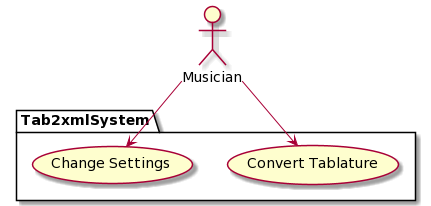
\includegraphics[width=.9\linewidth]{./Diagrams/use-case-diagram.png}
\end{center}
\section{User Stories}
\label{sec:orgd02b517}
\begin{enumerate}
\item "As a musician, I want to convert this text tablature to MusicXML so I can take advantage of MusicXML features like rendering, transposing and automatic playing."
\item "As a musician, I want to edit this text tablature if it is invalid so that I can ensure it is correct."
\end{enumerate}
\end{document}
